
\chapter{Testen und Validieren}
\label{chapter_Testen_und_Validieren}

Da das System in einem Langzeit-Teststand eingesetzt werden soll, ist die Zuverlässigkeit und die Betriebsfähigkeit über lange Zeiträume besonders wichtig. Es darf keine großen Performanceeinbußen oder lange Ausfälle beim Betrieb geben. In diesem Kapitel wird auf die Tests zur Sicherstellung dieser Kriterien eingegangen.

\section{Speicherlecks}

Ein häufiger Grund für Performanceeinbußen sind Speicherlecks (englisch: memory leak). Speicherlecks sind Fehler in der Programmierung der Speicherverwaltung, wodurch Speicher belegt, aber ungenutzt ist und nicht wieder freigegeben wird. Dabei kommt es zu einer immer größer werdenden Speichernutzung, bis der gesamte Speicher des Systems ausgelastet ist und es sich stark verlangsamt oder sogar Abstürzt.\\
Um Speicherlecks auszuschließen wurde die Steuerungssoftware mittels Valgrind \cite{valgrind} auf Speicherfehler überprüft. Dabei wurden alle Speicherlecks behoben.\\

\section{Stromausfall}

Nach einem Stromausfall muss das System binnen kürzester Zeit wieder einsatzbereit sein. Zur Sicherstellung dieser Eigenschaft wurden 20 Stromausfälle durch trennen und anschließend erneute verbinden der Stromversorgung simuliert.\\
Bei 20 Versuchen ist das System ohne Probleme neu gestartet. Das BeagleBone Black fährt bei Anschluss einer Stromversorgung automatisch hoch.

\section{Testaufbau}

Im Testaufbau werden zwei Mess-Clients an einen Mess-Server angeschlossen. Beiden Mess-Clients wurde vorher die RS232 Adresse 0 gegeben, damit sie sich bei dem Mess-Server anmelden können. Die Mess-Clients werden nach einander an des RS232 Bus angeschlossen und vom Mess-Server erkannt. Es ist dabei wichtig, zu warten bis der erste Mess-Client erfolgreich angemeldet ist, bevor der zweite Mess-Client angeschlossen ist. Würden beide Mess-Clients gleichzeitig angeschlossen werden, gebe es einen Adresskonflikt, da beide Mess-Clients die RS232 Adresse 0 besitzen.\\
Nach der erfolgreichen Anmeldung am Mess-Server, werden in den eingestellten Messintervallen die Messdaten aufgezeichnet. Über Desktop-Anwendung des PC-Clients kann auf die Mess-Clients zugegriffen werden. Die Messdaten können abgerufen und ausgewertet werden. Die Performance des Mess-Servers wird dabei nach durchgängigen Betrieb von 10 Tagen nicht beeinflusst. Lediglich bei einer Ansammlung von mehr als 500000 Messwerten werden die Datenbankabfragen langsamer.

\begin{figure}[H]
\begin{center}
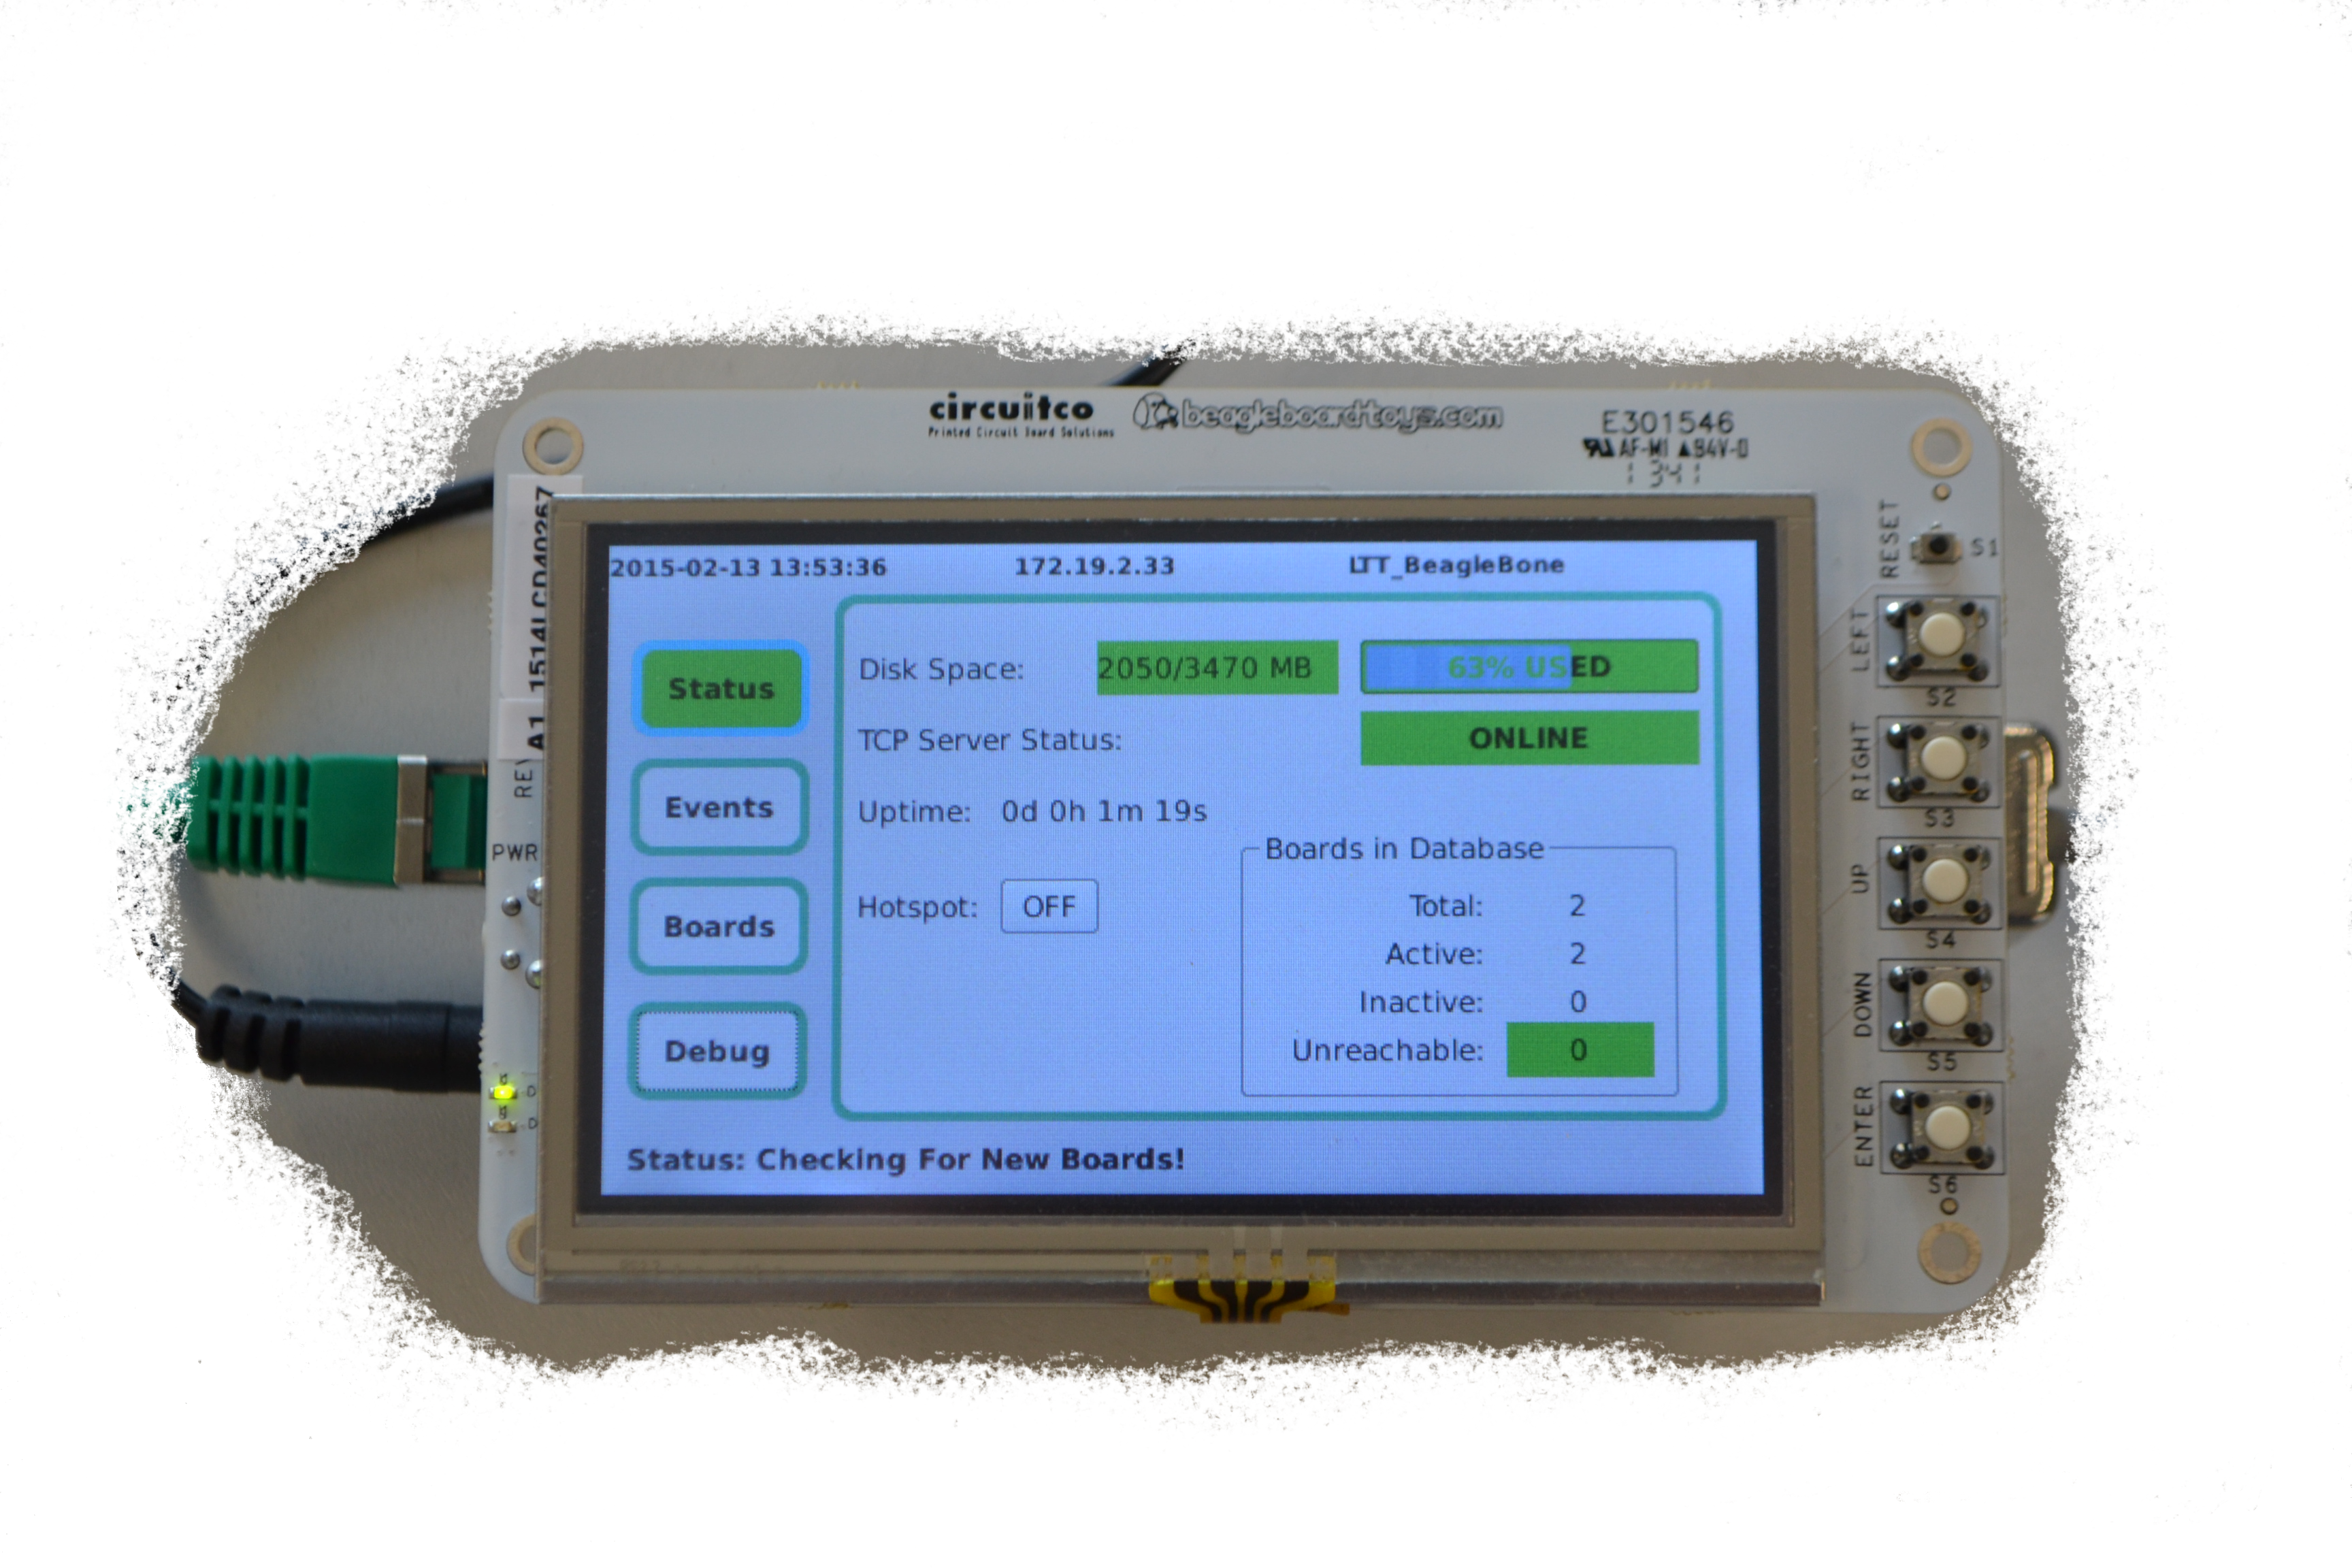
\includegraphics[width=0.7\textwidth]{img/general/MessServerAktiv.png}
\caption{Pulsmuster}
\label{figure_Pulsepattern}
\end{center}
\end{figure}
